\documentclass[11pt]{article}
\usepackage[toc,page]{appendix}
\usepackage{amsmath, amssymb}
\usepackage[utf8]{inputenc}
\usepackage[T1]{fontenc}
\usepackage[style=apa,backend=biber]{biblatex}
%\usepackage{biblatex}
\addbibresource{references.bib}
\usepackage{graphicx}
\usepackage{tikz}
\usetikzlibrary{automata,positioning,shapes.geometric, arrows.meta, fit, backgrounds, calc, chains}
\graphicspath{./images/Easy_Pictures/SMR_MULT_Repackaging}%\usepackage{kpfonts}
\usepackage{float}
\usepackage[margin=1in]{geometry}
\usepackage{cancel}
\usepackage{epsfig}
\usepackage{tikz-3dplot}
\usepackage{darkmode}
\usepackage{dirtytalk}
\usepackage{longtable,booktabs,array}
\usepackage{calc} % for calculating minipage widths
\usepackage[utf8]{inputenc}
\usepackage[T1]{fontenc}
\usepackage{xcolor}
\usepackage{listings}


\usepackage{etoolbox}
\usepackage{hyperref}
\hypersetup{
    colorlinks=true,
    linkcolor=blue,
    filecolor=magenta,      
    urlcolor=cyan,
    pdftitle={Hermeneutic Calculator},
    citecolor=blue,
    }


\urlstyle{same}

\lstdefinestyle{htmlStyle}{
    language=HTML,
    basicstyle=\ttfamily\small,
    keywordstyle=\color{blue}\bfseries,
    commentstyle=\color{gray}\itshape,
    stringstyle=\color{red},
    breaklines=true,
    frame=single,
    numbers=left,
    numberstyle=\tiny\color{gray},
    columns=fullflexible,
}
\lstdefinelanguage{HTML}{
  keywords={<!DOCTYPE, html, head, title, body, h1, h2, h3, p, div, span, a, img, ul, li, table, tr, td, th, style, link, script},
  sensitive=true,
  comment=[l]{//},
  morecomment=[s]{/*}{*/},
  morestring=[b]',
  morestring=[b]"
}
\lstset{style=htmlstyle, language=html}
% Updated to explicitly pass the language option
%\lstinputlisting[style=htmlstyle, language=html]{./html/example.html}
%\usepackage{tocloft}

% Optional: define some custom colors
\definecolor{sliceRed}{RGB}{225,224,91} % matching "varyellow" from your code
\definecolor{linkYellow}{RGB}{255,215,0}  % a golden yellow
\tdplotsetmaincoords{70}{110}

\title{Addition Strategies: Chunking by Bases and Ones}
\author{Compiled by: Theodore M. Savich}


\begin{document}
\maketitle
\subsection*{Transcript}
Strategy descriptions and examples adapted from \textcite{HackenbergCourseNotes}. Problem: Max  has  46  comic  books. For  his  birthday,  his  father  gives him  37  more  comic  books. How  many  comic  books  does  Max  have  now? 

\textbf{Dionne's solution:} ``He has 46. Then 37 more. {[}She writes
down 46, 76.{]} That's the 30. And then 7 more. Well, 4 more makes 80,
and then I only need to do 3 more, 83.''


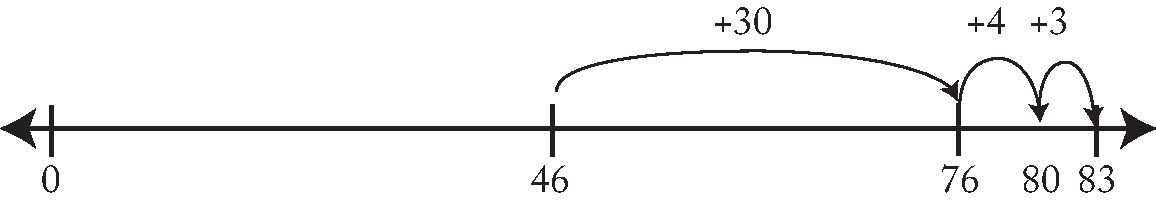
\includegraphics[width=.8\textwidth]{images/Easy_Pictures/SAR_ADD_CHUNKING/PDF/SAR_ADD_CHUNKING.pdf}

\noindent \textbf{Notation Representing Sarah's Solution:}

\begin{align*}
46 + 37 &= \Box \\
46 + 30 &= 76\\
76 + 4  &= 80\\
80+3 &= 83
\end{align*}

\subsubsection*{Description of Strategy:}

 \textbf{Objective:} Begin with one number. Then, break the other number down into bases and units. In COBO, you count on each base individually - then the ones. With Chunking, instead of adding each base individually, add them in well-chosen, larger groups. Likewise, combine the units in groups rather than one by one—though there are instances when adding a single base or unit makes strategic sense. The overall goal is to create larger, intentional groupings, and it’s important to clarify why each grouping is considered strategic. Usually, the goal with chunking on ones is to make a base first, then you can chunk on the rest of the ones. Usually when chunking on the bases, the goal is to make a base-of-bases first (so, in base ten, the goal would be to try and make one hundred), because then you can chunk on the rest of the bases (and ones) all at once. 

\subsubsection*{Description of Strategy}
\begin{itemize}
    \item \textbf{Objective:} Similar to COBO but add bases and ones in larger, strategic chunks.
    \item \textbf{Example:} \(46 + 37\)
    \begin{itemize}
        \item Start at \(46\).
        \item Add all tens at once: \(46 + 30 = 76\).
        \item Add ones strategically: \(76 + 4 = 80\), then \(80 + 3 = 83\).
    \end{itemize}
\end{itemize}

\subsubsection*{Automaton Type}
\textbf{Finite State Automaton (FSA)} with basic arithmetic capability.

\subsubsection*{Formal Description of the Automaton}

We define the automaton as the tuple
\[
M = (Q,\,\Sigma,\,\delta,\,q_{0/accept},\,F)
\]
where:
\begin{itemize}
    \item \(Q = \{q_{0/accept},\, q_1,\, q_2\}\) is the set of states.
    \item \(\Sigma = \{0,1,2,3,4,5,6,7,8,9,+\}\) is the input alphabet.
    \item \(q_{0/accept}\) is the start state, which is also the accept state.
    \item \(F = \{q_{0/accept}\}\) is the set of accepting states.
    \item The transition function \(\delta\) is defined as:
    \begin{enumerate}
        \item \(\delta(q_{0/accept},\, \text{``}A,B\text{''}) = q_1\) \quad with the action: set \(\text{Sum} \gets A\) and extract the base and ones chunks from \(B\).
        \item \(\delta(q_1,\, \varepsilon) = q_2\) \quad with the action: update \(\text{Sum} \gets \text{Sum} +\) (the bases chunk from \(B\)).
        \item \(\delta(q_2,\, \varepsilon) = q_2\) \quad with the action: if ones remain, add a strategic ones chunk to \(\text{Sum}\) (loop as needed).
        \item \(\delta(q_2,\, \varepsilon) = q_{0/accept}\) \quad with the action: when ones are finished, output \(\text{Sum}\).
    \end{enumerate}
\end{itemize}

\subsubsection*{Automaton Diagram for Chunking by Bases and Ones}

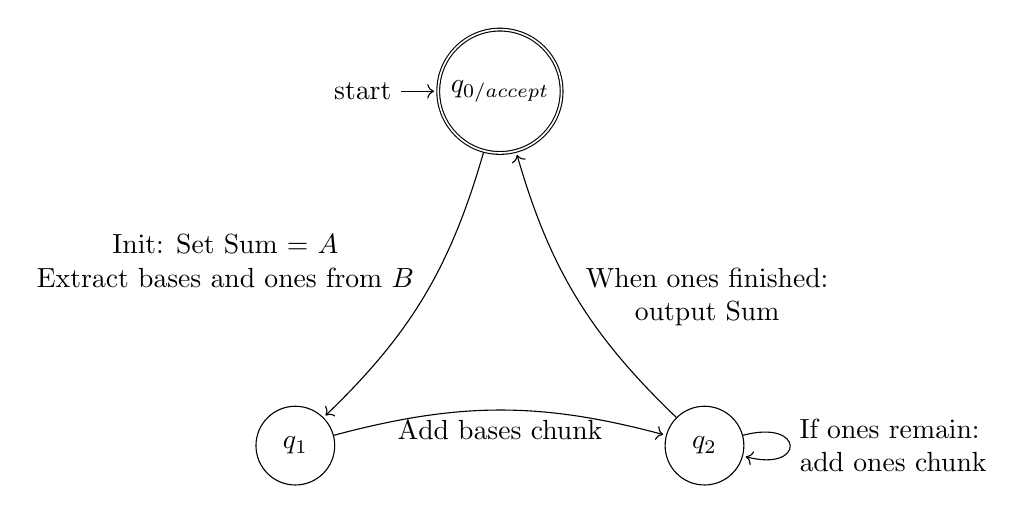
\begin{tikzpicture}[
    shorten >=1pt,
    auto,
    node distance=3cm,
    every state/.style={minimum size=1cm}
]
    % Arrange three states in a circle
    \node[state, initial, accepting] (q0) at (90:3cm) {$q_{0/accept}$};
    \node[state] (q1) at (210:3cm) {$q_1$};
    \node[state] (q2) at (330:3cm) {$q_2$};

    % Transition from q0 to q1
    \path[->]
        (q0) edge[bend left=15] node[above left, align=center] {Init: Set Sum = \(A\)\\Extract bases and ones from \(B\)} (q1)
    % Transition from q1 to q2
        (q1) edge[bend left=15] node[below, align=center] {Add bases chunk} (q2)
    % Loop on q2
        (q2) edge[loop right, looseness=8] node[right, align=left, align=left] {If ones remain:\\add ones chunk} (q2)
    % Transition from q2 to q0 (merged start/accept)
        (q2) edge[bend left=15] node[right, align=center] {When ones finished:\\output Sum} (q0);
\end{tikzpicture}

\clearpage


\subsubsection*{HTML Implementation}
\lstinputlisting[style=htmlStyle, language=html]{./new_html/SAR_ADD_Chunking.html}

\printbibliography
\end{document}